In this chapter, we show a theoretical analysis of \WFD and \FFD algorithms
run-time upper bound. In Section \ref{section:wfd_complexity}, we discuss \WFD
and in Section \ref{section:ffd_complexity}, we discuss \FFD.

% \section{Introduction}
% In Chapter \ref{chap:results} we will show that both \WFD and \FFD algorithms
% have been empirically prooven to be very fast frontier detectors relatively to a
% State-of-the-Art frontier detector. In this section, we show a theoretical
% analysis of their run-time upper bound. We denote $t$ as the time when a
% frontier detection algorithm was called.
% %The following proof relates to all \FFD executions between two
% %map-events. 


\section{\WFD Complexity Analysis}
\label{section:wfd_complexity}
As shown in Chapter \ref{chap:wfd}, \WFD is based on Breadth-First
Search (\BFS) over the occupancy grid. Within every call to \WFD, it
scans all \openspace regions for frontier points. When a frontier
point is found, \WFD performs another Breadth-First Search in order to
extract its frontier. Regarding a graph $G=\term{V,E}$, the upper bound of \BFS
run-time is $\order{E+V}$, full proof can be found in \cite{Cormen2001}.
Therefore, complexity of scanning the \openspace regions is linear in size of
the area of the \openspace regions. Moreover, frontier points are always located
on the edges of the \openspace regions. Thus, extracting frontiers from given frontier points
is also linear in size of the perimeter of the \openspace region.  
Hence, \WFD's run-time complexity is linear in size of the area (denoted
$\mathcal{S}\term{\cdot}$) and perimeter ($\mathcal{P}\term{\cdot}$) of the
\openspace region and can be formulated as:
\begin{equation}\label{eq:wfd_general_complexity}
\order{\underbrace{\mathcal{S}\term{open-space}}_{area} +
\underbrace{\mathcal{P}\term{open-space}}_{perimeter}}
\end{equation}

In the following sections we discuss \WFD's best case and worst
case. The reader should be aware to the fact that for a given map and a time
stamp, the \openspace area is determined by the trajectory of the robot.
However, its perimeter length affects the run-time and two cases
should be examined:

\subsection{\WFD Best Case}
The perimeter of the \openspace regions is minimal relatively to
the area of the \openspace regions. This can be shown in Figure
\ref{fig:wfd_best_case}.
\begin{figure}
  \centering
  \def\bgColor{gray!15}

\def\createBackground{% The graphic
  \draw[fill=\bgColor] (-1.2,-1.2) -- (1.2,-1.2) -- (1.2,1.2) -- (-1.2,1.2) --
  (-1.2,-1.2);
 }


\definecolor{myColor}{RGB}{94,38,18}
\def\emphColor{myColor}
\def\arrowWidth{1pt}	
\begin{tikzpicture}[scale=\MyTikzScale,cap=round]
	  % Local definitions
	  \def\costhirty{0.8660256}
	  \def\cosforthyfive{0.7071067811}
	  % Colors
	  \colorlet{coscolor}{blue}
	
	  % Styles
	  \tikzstyle{axes}=[]
	  \tikzstyle{important line}=[very thick]
	  %\tikzstyle{information text}=[rounded corners,fill=red!10,inner sep=1ex]
	
	  % The graphic
	  %\draw[style=help lines,step=0.5cm] (-1.4,-1.4) grid (1.4,1.4);
	\createBackground 
	\draw[line width=1pt,dashed,fill=white] (0,0) circle (1cm);
	    
	   \draw[style=important line,coscolor]
	    (0,0) -- node[right=2pt,fill=none] {$r$}
	    (0,1);
	\end{tikzpicture}

	\caption{\WFD Best Case: perimeter of \emph{open-space} regions
	is small as possible}
	\label{fig:wfd_best_case}
\end{figure}
In this case we denote the area of the shape as $S_{open}$ and its perimeter as
$P_{opt}$. Their values are shown in Equations \eqref{eq:S_opt} and
\eqref{eq:P_opt}:
\begin{equation}\label{eq:S_opt}
S_{open} = 4\pi r^2
\end{equation}

\begin{equation}\label{eq:P_opt}
P_{opt} = 2\pi r
\end{equation}

\subsection{\WFD Worst Case}
In the worst case we would like to maximize the length of the perimeter while
keeping the total area of the \openspace regions. Therefore we use a polygon as
an approximation to a circle. We take an inner regular polygon and build
triangles on each side. The level of accuracy is determined by $k$, the number
of vertices.
For a given $k$ value we denote the total area of the shape by $S_k$ and the
total perimeter length by $P_k$. In order to bound an area, at least 3
vertices have to be used. As previously mentioned, all areas are equal and thus,
for each $k \in \mathbb{N}\setminus\left\{0,1,2\right\}$ holds: $S_k = S_{open}$.
Figure \ref{fig:wfd_worst_case_polygons} demonstrates the results of different
$k$ values.

\begin{figure}
 \centering
 \subfigure[$k=4$] {
	 \def\bgColor{gray!15}

\def\createBackground{% The graphic
  \draw[fill=\bgColor] (-1.2,-1.2) -- (1.2,-1.2) -- (1.2,1.2) -- (-1.2,1.2) --
  (-1.2,-1.2);
 }


\definecolor{myColor}{RGB}{94,38,18}
\def\emphColor{myColor}
\def\arrowWidth{1pt}
\begin{tikzpicture}[scale=\MyTikzScale,cap=round]
  % Local definitions
  \def\costhirty{0.8660256}
  \def\cosforthyfive{0.7071067811}
  % Colors
  \colorlet{coscolor}{blue}

  % Styles
  \tikzstyle{axes}=[]
  \tikzstyle{important line}=[very thick]
  %\tikzstyle{information text}=[rounded corners,fill=red!10,inner sep=1ex]

  \createBackground
    
%     \path (-0.2,-0.2) coordinate (A) (0.2,-0.2) coordinate (B)
%           (0.2,0.2) coordinate (C) (-0.2,0.2) coordinate (D);
%         \draw[fill=white] (A)--(B)--(C)--(D)--cycle;
        
    \newdimen \R
    \R=0.4cm
     \draw[fill=white] (45:\R) \foreach \x in {0,45,135,...,405} {
     	-- (\x:\R)
     } -- cycle (135:\R);

   \draw[style=important line,coscolor]
    (0,0) -- node[right=2pt,fill=none] {$r$}
    (90:\R);
    
    
    
    
    \foreach \x in {45,135,...,405} {
%  		\prev=67.5;
     	\path (\x:\R) coordinate (P1) ;
     	\path (45+\x:\R+0.7cm) coordinate (P2);
     	\path (90+\x:\R) coordinate (P3);
     	\draw[fill=white, dashed, line width=1pt] (P1) -- (P2) -- (P3);
    }
% 	\draw[fill=white] (22.5:\R) \foreach \x in {67.5,112.5,...,382.5} {
%      	-- (\x:\R)
%      }	
    
    %\draw[fill=white, line width=1pt,dashed] (A)--(0,-1.2)--(B);
    %\draw[fill=white] (B)--(BC)--(C)--cycle;
    %\draw[fill=white] (C)--(CD)--(D)--cycle;
    %\draw[fill=white] (D)--(DA)--(A)--cycle;

    \draw[style=important line,\emphColor]
    (-45:\R) -- node[left=0pt,fill=none] {}
    (45:\R);
    
    \draw[\emphColor]
    (\R-0.11cm,0) -- node[left=5pt,above=0pt,fill=none] {}
    (0.7cm+\R,0);
    
    \node[anchor=east] at (\R+\R,0) (src_h) {};
  	\node[color=\emphColor,anchor=west] at (45:1.3cm) (dst_h) {$h_{4}$};
  	\node[anchor=east] at (-30:0.866*\R) (src_b) {};
  	\node[color=\emphColor,anchor=west] at (-45:1.3cm) (dst_b) {$b_{4}$};
  	\draw[\emphColor,line width=\arrowWidth] (dst_h) edge[out=180,in=0,<->]
  	(src_h); 
  	\draw[\emphColor,line width=\arrowWidth] (dst_b) edge[out=180,in=0,<->]
  	(src_b);
  	
  	\node[anchor=east] at (\R*0.5,1.5*\R) (src_l) {};
  	\node[color=\emphColor,anchor=west] at (65.5:1.1cm) (dst_l) {$l_{4}$};
  	\draw[\emphColor,line width=\arrowWidth] (dst_l) edge[out=180,in=0,<->]
  	(src_l); \draw[fill=white, \emphColor,line width=2pt] (P1) -- (P2); %l4
  	
%     \draw[style=important line,red]
%     (0.3cm,0) -- node[left=5pt,above=0pt,fill=none] {$h_4$}
%     (2.6*\R,0);
    
\end{tikzpicture}
	 \label{fig:polygon_4}
 }
 \subfigure[$k=8$] {
	 \def\bgColor{gray!15}

\def\createBackground{% The graphic
  \draw[fill=\bgColor] (-1.2,-1.2) -- (1.2,-1.2) -- (1.2,1.2) -- (-1.2,1.2) --
  (-1.2,-1.2);
 }


\definecolor{myColor}{RGB}{94,38,18}
\def\emphColor{myColor}
\def\arrowWidth{1pt}
\begin{tikzpicture}[scale=\MyTikzScale,cap=round]
  % Local definitions
  \def\costhirty{0.8660256}
  \def\cosforthyfive{0.7071067811}
  % Colors
  \colorlet{coscolor}{blue}

  % Styles
  \tikzstyle{axes}=[]
  \tikzstyle{important line}=[very thick]
  %\tikzstyle{information text}=[rounded corners,fill=red!10,inner sep=1ex]

 	\createBackground   
    
    
    \newdimen \R
    \R=0.4cm
     \draw[fill=white] (22.5:\R) \foreach \x in {67.5,112.5,...,382.5} {
     	-- (\x:\R)
     } -- cycle (112.5:\R);

   \draw[style=important line,coscolor]
    (0,0) -- node[right=2pt,fill=none] {$r$}
    (0,0.37);
    
    
    \foreach \x in {22.5,67.5,112.5,...,381.5} {
%  		\prev=67.5;
     	\path (\x:\R) coordinate (P1);
     	\path (22.5+\x:\R+0.7cm) coordinate (P2);
     	\path (45+\x:\R) coordinate (P3);
     	\draw[fill=white, dashed, line width=1pt] (P1) -- (P2) -- (P3);
     	
     	%\draw (P3) -- (P1);
%      	\path (\x:\R) coordinate (x2\x)
    	%\path (0.5*\x+0.5*(\x+45):\R) coordinate (curr)
    	%\draw[fill=white] (prev) -- (curr)
    	%\draw[fill=white] (\x:\R) -- (\x:\R);
    	%\draw (0.5*(\prev+\x):\R) -- (\x:\R);
    }
    
% 	\draw[fill=white] (22.5:\R) \foreach \x in {67.5,112.5,...,382.5} {
%      	-- (\x:\R)
%      }	
    
    %\draw[fill=white, line width=1pt,dashed] (A)--(0,-1.2)--(B);
    %\draw[fill=white] (B)--(BC)--(C)--cycle;
    %\draw[fill=white] (C)--(CD)--(D)--cycle;
    %\draw[fill=white] (D)--(DA)--(A)--cycle;
\draw[style=important line,\emphColor]
    (-22.5:\R) -- node[left=0pt,fill=none] {}
    (22.5:\R);
    
%     \draw[style=important line,red]
%     (0:\R+0.1) -- node[left=10pt,above=1pt,fill=none] {$h_8$}
%     (\R+0.60cm,0);
    
    \draw[\emphColor]
    (\R-0.03cm,0) -- node[left=5pt,above=-5pt,fill=none] {}
    (0.7cm+\R,0);

	\node[anchor=east] at (\R+\R,0) (src_h) {};
  	\node[color=\emphColor,anchor=west] at (45:1.3cm) (dst_h) {$h_{8}$};
  	\node[anchor=east] at (-10:\R) (src_b) {};
  	\node[color=\emphColor,anchor=west] at (-45:1.3cm) (dst_b) {$b_{8}$};
  	\draw[\emphColor,line width=\arrowWidth] (dst_h) edge[out=180,in=0,<->]
  	(src_h); 
  	\draw[\emphColor,line width=\arrowWidth] (dst_b)
  	edge[out=180,in=0,<->] (src_b);
    
    \node[anchor=east] at (\R*0.35,1.5*\R) (src_l) {};
  	\node[color=\emphColor,anchor=west] at (67.5:1.1cm) (dst_l) {$l_{8}$};
  	\draw[\emphColor,line width=\arrowWidth] (dst_l) edge[out=180,in=0,<->]
  	(src_l); 
  	\draw[fill=white, \emphColor,line width=\arrowWidth] (67.5:\R) -- (90:\R+0.7cm); %l8
    
\end{tikzpicture}

	 \label{fig:polygon_8}
 }
 \subfigure[$k=16$] {
	 \def\bgColor{gray!15}

\def\createBackground{% The graphic
  \draw[fill=\bgColor] (-1.2,-1.2) -- (1.2,-1.2) -- (1.2,1.2) -- (-1.2,1.2) --
  (-1.2,-1.2);
 }


\definecolor{myColor}{RGB}{94,38,18}
\def\emphColor{myColor}
\def\arrowWidth{1pt}
\begin{tikzpicture}[scale=\MyTikzScale,cap=round]
  % Local definitions
  \def\costhirty{0.8660256}
  \def\cosforthyfive{0.7071067811}
  % Colors
  \colorlet{coscolor}{blue}

  % Styles
  \tikzstyle{axes}=[]
  \tikzstyle{important line}=[very thick]
  %\tikzstyle{information text}=[rounded corners,fill=red!10,inner sep=1ex]

	\createBackground    
%     \path (-0.2,-0.2) coordinate (A) (0.2,-0.2) coordinate (B)
%           (0.2,0.2) coordinate (C) (-0.2,0.2) coordinate (D);
%         \draw[fill=white] (A)--(B)--(C)--(D)--cycle;
    
    % top triangle
    \path (0,-1.2) coordinate (ABC) (1.2,0) coordinate (BC)
          (0,1.2) coordinate (CD) (-1.2,0) coordinate (DA);
    
    \newdimen \R
    \R=0.4cm
     \draw[fill=white] (11.25:\R) \foreach \x in {33.75,56.25,...,371.25} {
     	-- (\x:\R)
     } -- cycle (101.25:\R);

   \draw[style=important line,coscolor]
    (0,0) -- node[right=2pt,fill=none] {$r$}
    (90:\R);
    
    
    \foreach \x in {33.75,56.25,...,371.25}{%{22.5,67.5,112.5,...,381.5} {
%  		\prev=67.5;
     	\path (\x:\R) coordinate (P1);
     	\path (11.25+\x:\R+0.7cm) coordinate (P2);
     	\path (22.5+\x:\R) coordinate (P3);
     	\draw[fill=white, dashed, line width=1pt] (P1) -- (P2) -- (P3);
     	
     	%\draw (P3) -- (P1);
%      	\path (\x:\R) coordinate (x2\x)
    	%\path (0.5*\x+0.5*(\x+45):\R) coordinate (curr)
    	%\draw[fill=white] (prev) -- (curr)
    	%\draw[fill=white] (\x:\R) -- (\x:\R);
    	%\draw (0.5*(\prev+\x):\R) -- (\x:\R);
    }
    
% 	\draw[fill=white] (22.5:\R) \foreach \x in {67.5,112.5,...,382.5} {
%      	-- (\x:\R)
%      }	
    
    %\draw[fill=white, line width=1pt,dashed] (A)--(0,-1.2)--(B);
    %\draw[fill=white] (B)--(BC)--(C)--cycle;
    %\draw[fill=white] (C)--(CD)--(D)--cycle;
    %\draw[fill=white] (D)--(DA)--(A)--cycle;
\draw[style=important line,\emphColor]
    (-11.25:\R) -- node[left=0pt,fill=none] {}
    (11.25:\R);
    
%     \draw[style=important line,red]
%     (0:\R+0.1) -- node[left=10pt,above=1pt,fill=none] {$h_8$}
%     (\R+0.60cm,0);
    
    \draw[\emphColor]
    (\R-0.01cm,0) -- node[left=5pt,above=-5pt,fill=none] {}
    (0.7cm+\R,0);
    
    \node[anchor=east] at (\R+\R,0) (src_h) {};
  	\node[color=\emphColor,anchor=west] at (45:1.3cm) (dst_h) {$h_{16}$};
  	\node[anchor=east] at (-5:\R) (src_b) {};
  	\node[color=\emphColor,anchor=west] at (-45:1.3cm) (dst_b) {$b_{16}$};
  	\draw[\emphColor,line width=\arrowWidth] (dst_h) edge[out=180,in=0,<->]
  	(src_h); 
  	\draw[\emphColor,line width=\arrowWidth] (dst_b) edge[out=180,in=0,<->]
  	(src_b);
    
    \node[anchor=east] at (\R*0.20,1.5*\R) (src_l) {};
  	\node[color=\emphColor,anchor=west] at (80:1.1cm) (dst_l) {$l_{16}$};
  	\draw[\emphColor,line width=\arrowWidth] (dst_l) edge[out=180,in=0,<->]
  	(src_l); \draw[fill=white, \emphColor,line width=2pt] (78.75:\R) -- (90:\R+0.7cm); %l8
    
\end{tikzpicture}

	 \label{fig:polygon_16}
 }
 \subfigure[$k=32$] {
	 \def\bgColor{gray!15}

\def\createBackground{% The graphic
  \draw[fill=\bgColor] (-1.2,-1.2) -- (1.2,-1.2) -- (1.2,1.2) -- (-1.2,1.2) --
  (-1.2,-1.2);
 }


\definecolor{myColor}{RGB}{94,38,18}
\def\emphColor{myColor}
\def\arrowWidth{1pt}
\begin{tikzpicture}[scale=\MyTikzScale,cap=round]
  % Local definitions
  \def\costhirty{0.8660256}
  \def\cosforthyfive{0.7071067811}
  % Colors
  \colorlet{coscolor}{blue}

  % Styles
  \tikzstyle{axes}=[]
  \tikzstyle{important line}=[very thick]
  %\tikzstyle{information text}=[rounded corners,fill=red!10,inner sep=1ex]

  % The graphic
  \createBackground   
    
%     \path (-0.2,-0.2) coordinate (A) (0.2,-0.2) coordinate (B)
%           (0.2,0.2) coordinate (C) (-0.2,0.2) coordinate (D);
%         \draw[fill=white] (A)--(B)--(C)--(D)--cycle;
        
    \newdimen \R
    \R=0.4cm
    
     \draw[fill=white] (5.625:\R) \foreach \x in {16.875,22.56,...,365.62} {
     	-- (\x:\R)
     } -- cycle (95.625:\R);

   \draw[style=important line,coscolor]
    (0,0) -- node[right=2pt,fill=none] {$r$}
    (90:\R);
    
    
    \foreach \x in {5.625,11.25,...,365.62} {
%  		\prev=67.5;
     	\path (\x:\R) coordinate (P1);
     	\path (5.625+\x:\R+0.7cm) coordinate (P2);
     	\path (11.25+\x:\R) coordinate (P3);
     	\draw[fill=white, dashed, line width=1pt] (P1) -- (P2) -- (P3);
     	
     	%\draw (P3) -- (P1);
%      	\path (\x:\R) coordinate (x2\x)
    	%\path (0.5*\x+0.5*(\x+45):\R) coordinate (curr)
    	%\draw[fill=white] (prev) -- (curr)
    	%\draw[fill=white] (\x:\R) -- (\x:\R);
    	%\draw (0.5*(\prev+\x):\R) -- (\x:\R);
    }
    
% 	\draw[fill=white] (22.5:\R) \foreach \x in {67.5,112.5,...,382.5} {
%      	-- (\x:\R)
%      }	
    
    %\draw[fill=white, line width=1pt,dashed] (A)--(0,-1.2)--(B);
    %\draw[fill=white] (B)--(BC)--(C)--cycle;
    %\draw[fill=white] (C)--(CD)--(D)--cycle;
    %\draw[fill=white] (D)--(DA)--(A)--cycle;
\draw[style=important line,\emphColor]
    (-5.625:\R) -- node[left=0pt,fill=none] {$b_{32}$}
    (5.625:\R);
    
%     \draw[style=important line,red]
%     (0:\R+0.1) -- node[left=10pt,above=1pt,fill=none] {$h_8$}
%     (\R+0.60cm,0);
    
    \draw[\emphColor]
    (\R,0) -- node[left=5pt,above=-5pt,fill=none] {}
    (0:0.7cm+\R);
%     (\R-0.01cm,0) -- node[left=5pt,above=-5pt,fill=none] {$h_{32}$}
%     (0.7cm+\R,0);

  	\node[anchor=east] at (\R+\R,0) (src_h){};
  	\node[color=\emphColor,anchor=west] at (45:1.3cm) (dst_h) {$h_{32}$};
  	\node[anchor=east] at (\R,0) (src_b) {};
  	\node[color=\emphColor,anchor=west] at (-45:1.3cm) (dst_b) {$b_{32}$};
  	\draw[\emphColor,line width=\arrowWidth] (dst_h) edge[out=180,in=0,<->]
  	(src_h); \draw[\emphColor, line width=\arrowWidth] (dst_b)
  	edge[out=180,in=0,<->] (src_b);

    \node[anchor=east] at (\R*0.65,1.5*\R) (src_l) {};
  	\node[color=\emphColor,anchor=west] at (60:1.3cm) (dst_l) {$l_{32}$};
  	\draw[\emphColor,line width=\arrowWidth] (dst_l) edge[out=180,in=0,<->]
  	(src_l); 
  	\draw[fill=white, \emphColor,line width=2pt] (67.5:\R) -- (71.125:\R+0.7cm);
  	%l8
    
\end{tikzpicture}
	 \label{fig:polygon_32}
 }
 \caption{\WFD worst case: different values of $k$}
 \label{fig:wfd_worst_case_polygons}
\end{figure}


\subsubsection{The General Case}
Assuming we have a general shape with an arbitrary number of vertices, $k$ and a
radius, $r$.
Let $b_k$ be the base of the inner polygon that is located inside the \openspace
regions (examples can be found in Figure \ref{fig:wfd_worst_case_polygons}). The
length of base $b_k$ is given by the formula:
\begin{equation}\label{eq:b_k}
b_k = 2r\cdot\tan{\frac{\pi}{k}}
\end{equation}
Let $h_k$ be the %distance between the center of the polygon and 
%one of its inner bases. 
height of an outer triangle.
The length of $h_k$ is given by equation \eqref{eq:h_k}:
\begin{eqnarray}\label{eq:h_k}
S_k &=& S_{open} \nonumber\\
k\cdot\frac{r\cdot b_k}{2} + k\cdot\frac{h_k\cdot b_k}{2} &=& 4\pi r^2
\nonumber\\
k\cdot r\cdot b_k + k\cdot h_k\cdot b_k &=& 8\pi r^2 \nonumber\\
h_k = \frac{8\pi r^2 - k\cdot r\cdot b_k}{k\cdot b_k} &=& 
	  \frac{8\pi r^2}{k\cdot b_k} - r
\end{eqnarray}
Let $l_k$ be the length of an outer triangle side. The length of $l_k$ is given
by equation \eqref{eq:l_k}:
\begin{equation}\label{eq:l_k}
l_k = \sqrt{\term{h_k}^2 + \term{\frac{b_k}{2}}^2}
\end{equation}
Therefore, the length of the polygon's perimeter equals to the total
length of the outer edges of the triangles. We can calculate the
perimeter of the polygon by:
\begin{equation}
P_k = 2k\cdot l_k
\end{equation}
We now express the perimeter $P_k$ as a function of the area $S_{open}$:
\begin{eqnarray}\label{eq:P_to_S_1}
P_k &=& 2k\cdot l_k \nonumber\\
 &=& 2k\sqrt{\term{h_k}^2 + \term{\frac{b_k}{2}}^2} \nonumber\\
 &=& 2k\sqrt{\term{\frac{8\pi r^2}{k\cdot b_k} - r}^2 +
 \term{\frac{2r\cdot\tan{\frac{\pi}{k}}}{2}}^2} \nonumber\\
 &=& 2k\sqrt{\term{\frac{8\pi r^2}{k\cdot b_k} - r}^2 +
 \term{r\cdot\tan{\frac{\pi}{k}}}^2}
\end{eqnarray} 
Equations \eqref{eq:S_opt} and \eqref{eq:b_k} can be joint with Equation
\eqref{eq:P_to_S_1}:
\begin{eqnarray}\label{eq:P_to_S_2}
P_k &=& 2k\sqrt{\term{\frac{2S_{open}}{k\cdot 2r\cdot\tan{\frac{\pi}{k}}} - r}^2 +
 \term{r\cdot\tan{\frac{\pi}{k}}}^2} \nonumber \\
&=& 2k\sqrt{\term{\frac{S_{open}}{k\cdot r\cdot\tan{\frac{\pi}{k}}} - r}^2 +
 \term{r\cdot\tan{\frac{\pi}{k}}}^2} \nonumber\\
&=& 2k\sqrt{\term{\frac{S_{open}}{k\cdot r\cdot\tan{\frac{\pi}{k}}}}^2
	       -2\frac{r\cdot S_{open}}{k\cdot r\cdot\tan{\frac{\pi}{k}}}
	       + r^2 + 
 r^2\cdot\tan^2{\frac{\pi}{k}}} \nonumber\\
 &=& 2k\sqrt{\term{\frac{S_{open}}{k\cdot r\cdot\tan{\frac{\pi}{k}}}}^2
	       -2\frac{S_{open}}{k\cdot\tan{\frac{\pi}{k}}}
	       + r^2\term{1+\tan^2{\frac{\pi}{k}}}} \nonumber\\
&=& 2k\sqrt{\term{\frac{S_{open}}{k\cdot r\cdot\tan{\frac{\pi}{k}}}}^2
	       -2\frac{S_{open}}{k\cdot\tan{\frac{\pi}{k}}}
	       + \frac{r^2}{\cos^2{\frac{\pi}{k}}}} \nonumber\\
&=& \sqrt{\term{\frac{2k\cdot S_{open}}{k\cdot r\cdot\tan{\frac{\pi}{k}}}}^2
	       -2\frac{4k^2\cdot S_{open}}{k\cdot\tan{\frac{\pi}{k}}}
	       + \frac{4k^2\cdot r^2}{\cos^2{\frac{\pi}{k}}}} \nonumber\\
&=& \sqrt{\term{\frac{2\cdot S_{open}}{r\cdot\tan{\frac{\pi}{k}}}}^2
	       -8\frac{k\cdot S_{open}}{\tan{\frac{\pi}{k}}}
	       + 4\frac{k^2\cdot r^2}{\cos^2{\frac{\pi}{k}}}}
\end{eqnarray} 
The only case that yields a division by zero in Equation \eqref{eq:P_to_S_2}
happens when $k=2$. That causes both $\tan{\frac{\pi}{k}}$ and
$\cos{\frac{\pi}{k}}$ to return the value of $\infty$. In any other values of
$k$, the functions are well-defined. Since we work on a discrete domain, the
number of vertices the polygon that approximate the \openspace area is bounded
by the number of \openspace points, which in our case equals to $S_{open}$:
\begin{equation}\label{eq:bound_k_to_S}
	k \le S_{open}
\end{equation}
In the range $\left[3,\infty\right)$ the function $f(x)=\frac{1}{\cos{x}}$
is a monotonic deceasing function and therefore gets a maximal value of 2. This
yields:
\begin{equation}\label{eq:bound_cosine}
	\frac{1}{\cos{\frac{\pi}{k}}} \le 2 \qquad{ \text{for } k \in
	\mathbb{N}\setminus\left\{0,1,2\right\}}
\end{equation}
 Therefore, Equations \eqref{eq:P_to_S_2},
 \eqref{eq:bound_k_to_S} and \eqref{eq:bound_cosine} can be joint and we get
 Equation \eqref{eq:P_to_S_3}:
\begin{equation}\label{eq:P_to_S_3}
P_k \le \sqrt{\term{\frac{2\cdot S_{open}}{r\cdot\tan{\frac{\pi}{S_{open}}}}}^2
	       -8\frac{S_{open}^2}{\tan{\frac{\pi}{S_{open}}}}
	       + 2\cdot S_{open}^2\cdot r^2}
\end{equation}
Therefore, when we join Equation
\eqref{eq:P_to_S_3} together with \eqref{eq:wfd_general_complexity}, we get the
overall run-time complexity of \WFD algorithm in terms of the \openspace area,
$S_{open}$:
\begin{equation*}
\order{S_{open} +
\sqrt{\term{\frac{2\cdot
S_{open}}{r\cdot\tan{\frac{\pi}{S_{open}}}}}^2
-8\frac{S_{open}^2}{\tan{\frac{\pi}{S_{open}}}} + 2\cdot S_{open}^2\cdot r^2
	 }
}
\end{equation*}
After omitting constants:
\begin{equation}\label{eq:wfd_final_complexity}
\order{S_{open} +
\sqrt{\term{\frac{
S_{open}}{r\cdot\tan{\frac{\pi}{S_{open}}}}}^2
-\frac{S_{open}^2}{\tan{\frac{\pi}{S_{open}}}} + S_{open}^2\cdot r^2
	 }
}
\end{equation}


\begin{figure}
\centering
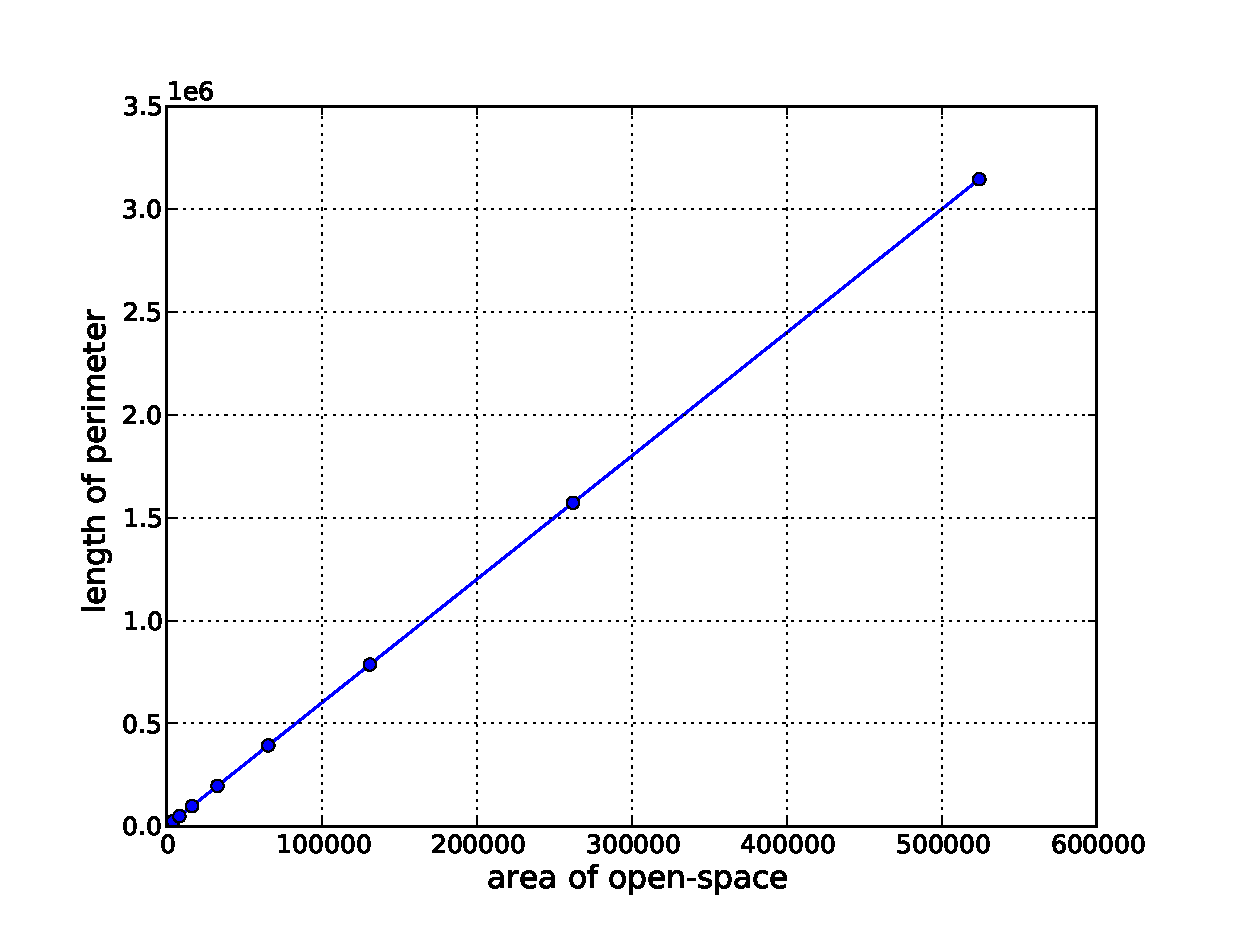
\includegraphics[width=0.6\columnwidth,keepaspectratio]{images/perimeter_graph.eps}
\caption{The linearity relation between the area of \openspace region
and its perimeter (Equation \eqref{eq:P_to_S_2}). The x-axis contains samples of
different \openspace regions in sizes of: $2^2,2^3,\ldots,2^{20}$ and y-axis contains their perimeter size,
respectively.}
\label{fig:linearity_of_perimeter_length}
\end{figure}


\begin{figure}
\centering
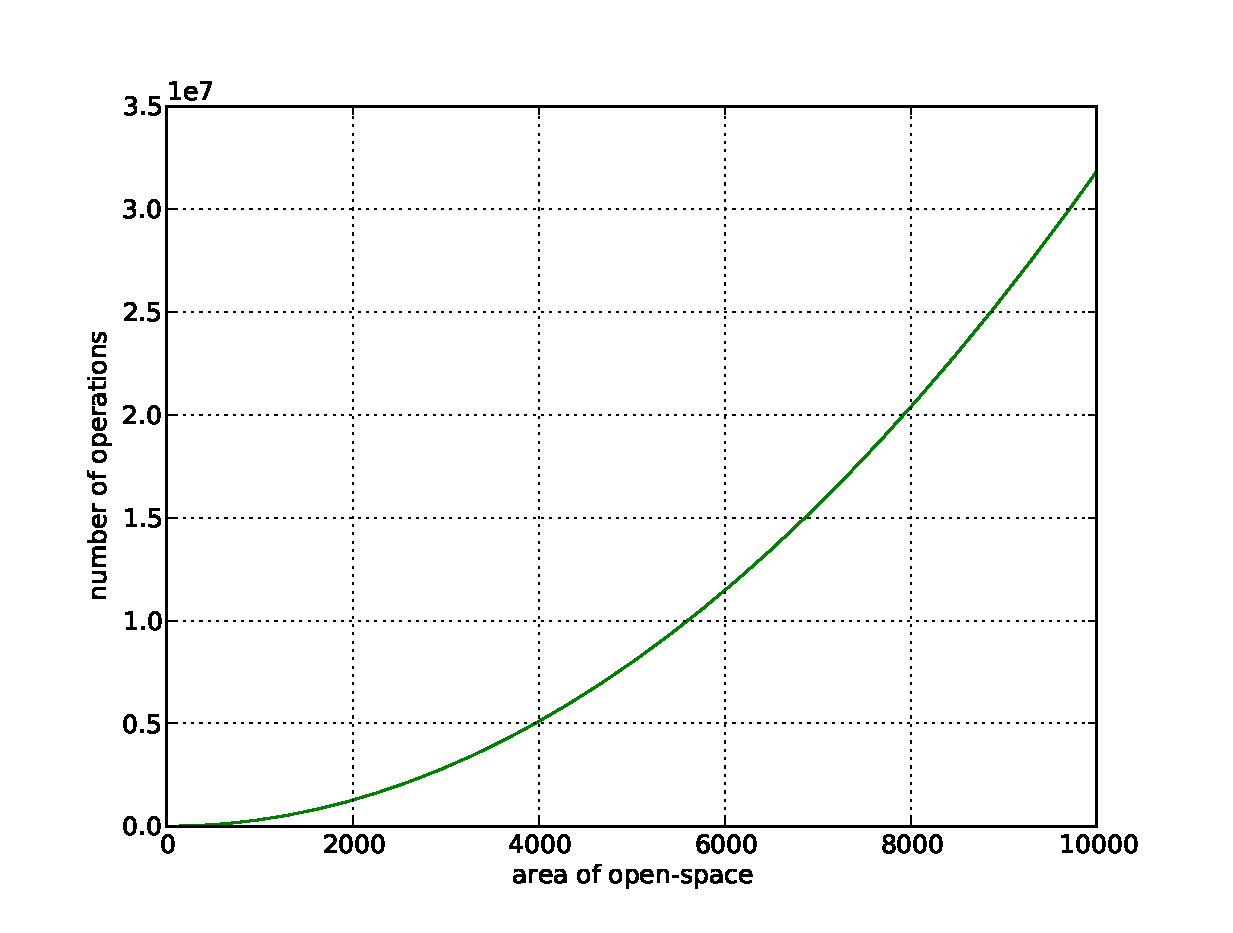
\includegraphics[width=0.6\columnwidth,keepaspectratio]{images/wfd_comp.eps}
\caption{\WFD's complexity function, Equation \eqref{eq:wfd_final_complexity}
}
\label{fig:wfd_final_complexity}
\end{figure}

Figure \ref{fig:linearity_of_perimeter_length} shows an evaluation of the
\openspace region's perimeter length as a function of the total area of
\openspace regions.

Figure \ref{fig:wfd_final_complexity} shows the graph for \WFD final complexity
function (Equation \eqref{eq:wfd_final_complexity}), in the range
of $S_{open} \in \left[0,10000\right]$.

%\section{Comparing \WFD to \FFD}

%We also showed that the run-time
%complexity of \FFD is bounded by $\order{\execTime{c} + log{\execTime{n_f}}}$,
%full proof can be found in Section \ref{section:ffd_complexity}.

%\NOTE{The following is a draft, but should clarify the point}
%In the worst case of \emph{FFD}, the size of the contour is almost equal to the
%area of the active area. In contrary, if \WFD is executed in the same point in
%time, it has to process the entire \openspace regions. Thus, \WFD is not better
%than \FFD because the entire active area is counted as an \openspace region.

\section{\FFD Complexity Analysis}
\label{section:ffd_complexity}
In Section \ref{section:wfd_complexity}, we showed that the run-time complexity
of \WFD is bounded by Equation \eqref{eq:wfd_general_complexity}.
Allegedly, it may seem that \FFD's complexity is contained within \WFD since
\FFD searches only inside the active area where all of its points are
\openspace. However, this is not true since \FFD has to persistently run in the
background. It may thus run a number of times by every single run of \WFD.
Moreover, it run for each particle, in particle-based mapping systems.
As shown in Chapter \ref{chap:ffd}, \FFD contains four stages.
We now analyse the complexity of each stage separately: 

\subsection{Sorting stage (Algorithm \ref{alg:ffd_sorting_stage})}
\FFD performs polar-sorting of laser readings. 
\FFD utilizes cross-product instead of actually
calculating angle and radius (which are relatively
very time-consuming calculations). As explained in Chapter
\ref{chap:ffd}, in order to determine the order of the points
received from the laser readings, we calculate the cross-product between
them. Cross-product calculation is performed in a constant time and
sorting is performed in time of $\order{n\log{n}}$. We denote $l_r$ as
the number of laser readings received in each measurement and therefore, total
complexity of this stage is:
 \begin{equation}\label{eq:sorting}
 	\order{l_r\log{l_r}} \cdot \order{1} = \order{l_r \log{l_r}}
 \end{equation}

\subsection{Contour stage (Algorithm \ref{alg:ffd_contour_stage})}
%(Lines \ref{mark:ffd_contour_start}--\ref{mark:ffd_contour_end})}
\FFD scans each two adjacent points received from the polar-sorted laser
readings. For each two adjacent points \FFD calls \emph{Bresenham's line algorithm} which returns
a set of the points that lie between them. \emph{Bresenham's line algorithm} is
performed in linear time complexity. In the end, \FFD merges all received lines
into a single contour. We denote $d_{p_i,p_j}$ as the euclidean distance
between points $p_i$ and $p_j$. Therefore, total complexity of this stage is
the total distance between each two adjacent points, which is denoted as
$\execTime{c}$, the length of the contour in time $t$:
\begin{equation}\label{eq:contour}
\order{\sum_{p_i \in l_r}{d_{p_{i-1},p_i}}} = \order{\execTime{c}}
\end{equation}

\subsection{Detecting new frontiers stage (Algorithm \ref{alg:ffd_detect_new_frontier_stage})}
%(Lines \ref{mark:ffd_extract_start}--\ref{mark:ffd_extract_end})} 
\FFD scans the contour from the previous stage and extracts new frontiers (if
available of course).
Each found new detected frontier is added into a list (which will be used in
next stage) and hence, the addition is performed in a constant time. Lines
\ref{mark:ffd_extract_start}--\ref{mark:ffd_special_case_end} handle the
special case when the first point on the contour is a frontier point. All
actions are performed in a constant time. Therefore, total complexity of this
stage is proportional to the length of the given contour:
\begin{equation}\label{eq:detection}
	\underbrace{\order{1}}_{\textrm{special case}} +
	\underbrace{\order{\execTime{c}} \cdot \order{1}}_{\textrm{general case}} =
	\order{\execTime{c}}
\end{equation}

\subsection{Maintenance stage (Algorithm \ref{alg:ffd_maintenance_stage})}
%(Lines \ref{mark:ffd_maintenance_start}--\ref{mark:ffd_maintenance_end})}
\subsubsection{Elimination of previous frontiers (Lines
\ref{mark:ffd_eliminating_previous_frontiers_start}--\ref{mark:ffd_eliminating_previous_frontiers_end})}
\FFD scans each point which lies inside the active area and checks if it was
previously belonged to a frontier. Checking a specific point is performed in a
constant time since all points in map already store a frontier index. The index
is used as a lookup index in the frontier database (full implementation details
can be found in Chapter \ref{chap:ffd}). We denote $\execTime{A}$ as the bounding
rectangle (the active area) in time $t$. Hence, scanning all points in the
active area can be done in time of $\order{\execTime{A}} \cdot \order{1} =
\order{\execTime{A}}$. We denote $\execTime{f_{max}}$ as the length of the
longest frontier that exists in the frontier database in time $t$ and
$\execTime{n_f}$ as the number of frontiers that are stored in the frontier
database in time $t$. If a previously frontier point is found, then \FFD
searches for its frontier in the database and removes this point from the
frontier. Therefore, for a specific frontier point it takes
$\order{\log{\execTime{n_f}}}$ to find the frontier in the frontier database by
the lookup index (we used a self-balancing binary search tree in our
implementation), $\order{\execTime{f_{max}}}$ to locate the specific point in
the found frontier and $\order{1}$ to remove it from the found frontier.
Therefore, total complexity for this stage is:
\begin{equation}\label{eq:elimination}
	\order{\execTime{A}} \cdot
    \order{\execTime{f_{max}} +
        \log{\execTime{n_f}}}
    =
    \order{\execTime{A} \cdot
        \left(\execTime{f_{max}} +
        \log{\execTime{n_f}}\right)} 
\end{equation}

\subsubsection{Adding new frontiers (Lines
\ref{mark:ffd_storing_new_frontiers_start}--\ref{mark:ffd_storing_new_frontiers_end})}
\FFD scans each frontier point within all new detected frontiers that were found
at the detection stage. We denote $\execTime{n_{new}}$ as the number of new
frontiers that were found in time $t$ and hence, scanning all new detected
frontiers that are found in time $t$ is performed in complexity of
$\order{\execTime{n_{new}}}$. Next, \FFD checks if each new detected frontier
point belongs to another previously detected frontier. As mentioned before, this
check can be performed in a constant time since each point stores a frontier
lookup index. Therefore, scanning all points in a specific frontier is performed
in time of $\order{\execTime{f_{max}}}$ and searching the frontier whose index
is stored within the point is performed in time of
$\order{\log{\execTime{n_f}}}$. In the end, the new frontier is merged with the
existing frontier which is performed in a constant time. Total complexity of
this stage is:
\begin{equation}\label{eq:add_new_frontiers}
	\order{\execTime{n_{new}}} \cdot
  	\order{\execTime{f_{max}} + \log{\execTime{n_f}} } 
  	=
  	\order{\execTime{n_{new}} \cdot 
  		\term{\execTime{f_{max}} + \log{\execTime{n_f}}}}
\end{equation}

\subsection{Combining all stages}
By joining together equations: \eqref{eq:sorting}, \eqref{eq:contour},
\eqref{eq:detection}, \eqref{eq:elimination} and \eqref{eq:add_new_frontiers},
we get the total complexity for one iteration:
\begin{eqnarray}\label{eq:merged_2}
&&\order{ \underbrace{l_r\log{l_r}}_{\textrm{sorting}} + 
        \underbrace{\execTime{c}}_{\textrm{contour}} +
        \underbrace{\execTime{c}}_{\textrm{detection}} +
        \overbrace{\underbrace{\execTime{A} \cdot
                \term{\execTime{f_{max}} +
                \log{\execTime{n_f}}})}_{\textrm{eliminate
                existing frontiers}} + 
                \underbrace{\execTime{n_{new}} 
                \cdot \term{\execTime{f_{max}} + \log{\execTime{n_f}}
                }}_{\textrm{add new frontiers}}}^{\textrm{frontiers
                maintenance}} }
\nonumber \\
&=&\order{ l_r\log{l_r} + 
        \execTime{c} +
        \term{\execTime{A} + \execTime{n_{new}}}
        \cdot \term{\execTime{f_{max}} +
        \log{\execTime{n_f}}} }
\end{eqnarray}
All new detected frontiers are found only inside the active area. Thus, the
number of new detected frontiers is bounded by size of the active area:
\begin{equation}\label{eq:bound_new_frontiers}
\execTime{n_{new}} \le \execTime{A}
\end{equation}
All new detected frontiers lie within the contour. In the worst-case, all
points that lie within the contour belong to the longest frontier. Hence,
we can bound the length of the longest frontier by the contour's length:
\begin{equation}\label{eq:bound_frontier_length}
\execTime{f_{max}} \le \execTime{c}
\end{equation}
Therefore, by joining the upper bounds from equations
\eqref{eq:bound_new_frontiers} and
\eqref{eq:bound_frontier_length} together with \eqref{eq:merged_2} we bound the
complexity of \FFD by Equation \eqref{eq:merged_3} below:
\begin{eqnarray}\label{eq:merged_3}
&&\order{l_r\log{l_r} + 
        \execTime{c} +
        \term{\execTime{A} + \execTime{A}} \cdot
        \term{\execTime{c} +
        \log{\execTime{n_f}}} 
       } \nonumber \\
&=&\order{l_r\log{l_r} + 
        \execTime{c} +
        \execTime{A} \cdot
        \term{\execTime{c} +
        \log{\execTime{n_f}}}
        }
\end{eqnarray}
The size of the active area can be bounded by the maximum range of the laser.
The largest active area rectangle is received only when the the laser scans an open
area. In this case, the active area is a rectangle that bounds a circle whose
radius equals to the maximum laser range: 
\begin{equation} 
\label{eq:active_area_bound}
\execTime{A} \le \term{2l_{m}} \times \term{2l_{m}} =
4\term{l_{m}}^2
\end{equation} 
Joining together \eqref{eq:merged_3} and \eqref{eq:active_area_bound}:
\begin{eqnarray}
&&\order{l_r\log{l_r} + 
        \execTime{c} +
        4\term{l_{m}}^2 \cdot
        \term{\execTime{c} +
        \log{\execTime{n_f}}}
     } \nonumber \\
&=&\order{l_r\log{l_r} + 
        \execTime{c} +
        4\term{l_{m}}^2 \cdot \execTime{c} +
        4\term{l_{m}}^2 \cdot\log{\execTime{n_f}}} \nonumber \\      
&=&\order{l_r\log{l_r} + 
        \term{1+4\term{l_{m}}^2} \cdot \execTime{c} +
        4\term{l_{m}}^2 \cdot\log{\execTime{n_f}}}   
\end{eqnarray} 
The maximal laser range and the number of laser readings ($l_m$ and
$l_r$, respectively) do not change during the execution. Hence, they both 
can be considered as constants and therefore, can be removed from the
asymptotic upper bound:
\begin{equation}\label{eq:ffd_final_complexity_single_iteration}
\order{\execTime{c} +
        \log{\execTime{n_f}}}        
\end{equation}

\section{Summary}
In this chapter, we showed running-time upper-bounds for both \WFD and \FFD
algorithms (Section \ref{section:wfd_complexity} and Section
\ref{section:ffd_complexity}, respectively).
Until now, we discussed \FFD's run-time complexity in a single execution.
However, as said in Chapter \ref{chap:ffd}, \FFD has to persistently run in the
background. More precisely, in order to maintain previously detected frontiers,
\FFD is executed when a new laser reading is received. Traditional frontier
detectors are executed on demand, usually when a \emph{\mapevent} has occurred.
A \emph{\mapevent} is an event which is raised by the SLAM implementation
when a sufficient amount of new data was received in order to produce a new map.
In order to compare \FFD to other traditional frontier detectors, we define
$l_\omega$ as the frequency of the laser sensor (e.g. how many laser readings
are received in a time unit of 1 second). In addition, we denote $t_{m}$ to be
the worst-case elapsed time between two following map-events in the (i.e. in
times $t_i$ and $t_{i+1}$).  Finally, we denote $P_n$ as the number of particles
in the SLAM implementation. In implementations containing only one map, such as
EKF-based systems, the value of $P_n$ is 1. The reason is that as said in
Chapter \ref{chap:ffd}, each particle has to maintain its own map and thus, run
its own instance of \FFD. Thus, Equation
\eqref{eq:ffd_final_complexity_single_iteration} now considers the frequency of
the laser sensor and we get Equation \eqref{eq:ffd_complexity_with_freq}:
\begin{equation}\label{eq:ffd_complexity_with_freq}
\order{P_n\cdot \term{t_m \cdot l_\omega} \cdot\term{\execTime{c} +
        \log{\execTime{n_f}}}}
\end{equation}

It might seem that in Equation \eqref{eq:ffd_complexity_with_freq} the value of
$P_n\cdot \term{t_m \cdot l_\omega}$ is constant during all \FFD executions and
hence, redundant. However, in real-world situations, this value plays a major
role in determining \FFD's run-time. For example:
although lower values of $l_\omega$ decrease the number of \FFD executions in
the time between two following map-events, increasing the number of \FFD
instances (e.g. increasing the number of particles in a particle-filter based
SLAM implementation) causes the total run-time becoming slower. The question
remains open: how do $P_n$, $t_m$, and $l_\omega$ values affect \FFD's
run-time in the real-world?
The answer to this question is presented in Chapter \ref{chap:results}.

